\documentclass[12pt,a4paper]{article}
\usepackage[utf8]{inputenc}
\usepackage[T1]{fontenc}
\usepackage[english]{babel}
\usepackage{amsmath,amsfonts,amssymb}
\usepackage{graphicx}
\usepackage{xcolor}
\usepackage{tikz}
\usetikzlibrary{shapes,arrows,positioning,calc,fit}
\usepackage{listings}
\usepackage{fancyhdr}
\usepackage{geometry}
\usepackage{booktabs}
\usepackage{colortbl}
\usepackage{tcolorbox}
\usepackage{fontawesome5}

\geometry{margin=2.5cm}

% Colors
\definecolor{primaryblue}{RGB}{41,98,255}
\definecolor{secondarygreen}{RGB}{0,150,136}
\definecolor{accentorange}{RGB}{255,152,0}
\definecolor{darkgray}{RGB}{66,66,66}
\definecolor{lightgray}{RGB}{245,245,245}
\definecolor{codebg}{RGB}{40,44,52}

% Header/Footer
\pagestyle{fancy}
\fancyhf{}
\fancyhead[L]{\textcolor{primaryblue}{\textbf{Cryptography}}}
\fancyhead[R]{\textcolor{darkgray}{Ahmed Dinari}}
\fancyfoot[C]{\thepage}
\renewcommand{\headrulewidth}{2pt}
\renewcommand{\headrule}{\hbox to\headwidth{\color{primaryblue}\leaders\hrule height \headrulewidth\hfill}}

% Code listing style
\lstset{
    backgroundcolor=\color{codebg},
    basicstyle=\ttfamily\small\color{white},
    breaklines=true,
    frame=single,
    rulecolor=\color{primaryblue},
    numbers=left,
    numberstyle=\tiny\color{gray},
    keywordstyle=\color{accentorange},
    stringstyle=\color{secondarygreen},
    commentstyle=\color{gray},
}

% Custom boxes
\newtcolorbox{conceptbox}[1]{
    colback=lightgray,
    colframe=primaryblue,
    fonttitle=\bfseries,
    title=#1,
    rounded corners,
    boxrule=2pt
}

\newtcolorbox{importantbox}{
    colback=accentorange!10,
    colframe=accentorange,
    rounded corners,
    boxrule=2pt
}

\begin{document}

% ============================================================
% TITLE PAGE
% ============================================================
\begin{titlepage}
    \centering
    \vspace*{2cm}
    
    {\Huge\bfseries\textcolor{primaryblue}{Cryptography}\par}
    \vspace{0.5cm}
    {\LARGE\textcolor{darkgray}{Symmetric vs Asymmetric}\par}
    
    \vspace{2cm}
    
    \begin{tikzpicture}[scale=0.8]
        % Symmetric side
        \node[draw=secondarygreen, fill=secondarygreen!20, rounded corners, minimum width=4cm, minimum height=1.5cm] (sym) at (-4,0) {\textbf{Symmetric}};
        \node[circle, draw=secondarygreen, fill=secondarygreen!30, minimum size=1cm] (key1) at (-4,-2) {\faKey};
        \node[below=0.3cm of key1] {\small 1 Key};
        
        % Asymmetric side
        \node[draw=primaryblue, fill=primaryblue!20, rounded corners, minimum width=4cm, minimum height=1.5cm] (asym) at (4,0) {\textbf{Asymmetric}};
        \node[circle, draw=primaryblue, fill=primaryblue!30, minimum size=1cm] (key2) at (3,-2) {\faKey};
        \node[circle, draw=accentorange, fill=accentorange!30, minimum size=1cm] (key3) at (5,-2) {\faLock};
        \node[below=0.3cm of key2] {\small Public};
        \node[below=0.3cm of key3] {\small Private};
        
        % VS
        \node[circle, draw=darkgray, fill=white, minimum size=1.5cm] at (0,0) {\Large\textbf{VS}};
    \end{tikzpicture}
    
    \vspace{3cm}
    
    {\Large\textbf{Practical Demonstration}\par}
    \vspace{0.5cm}
    {\large File Encryption and Decryption\par}
    
    \vfill
    
    \begin{tabular}{rl}
        \textbf{Author:} & Ahmed Dinari \\
        \textbf{Date:} & November 2025 \\
        \textbf{Course:} & Computer Security \\
    \end{tabular}
    
\end{titlepage}

% ============================================================
% TABLE OF CONTENTS
% ============================================================
\tableofcontents
\newpage

% ============================================================
% INTRODUCTION
% ============================================================
\section{Introduction}

\textbf{Cryptography} is the art of protecting information by transforming it into an unreadable format for anyone who does not possess the decryption key.

\begin{conceptbox}{Objectives of Cryptography}
\begin{itemize}
    \item \textbf{Confidentiality}: Only authorized persons can read the message
    \item \textbf{Integrity}: The message has not been modified
    \item \textbf{Authentication}: The sender's identity is verified
    \item \textbf{Non-repudiation}: The sender cannot deny having sent the message
\end{itemize}
\end{conceptbox}

There are two main families of encryption:
\begin{enumerate}
    \item \textbf{Symmetric Encryption} (AES, DES, 3DES)
    \item \textbf{Asymmetric Encryption} (RSA, ECC, DSA)
\end{enumerate}

% ============================================================
% SYMMETRIC ENCRYPTION
% ============================================================
\section{Symmetric Encryption}

\subsection{Principle}

Symmetric encryption uses \textbf{a single key} to both encrypt AND decrypt data.

\begin{center}
\begin{tikzpicture}[node distance=2cm, auto]
    % Styles
    \tikzstyle{block} = [rectangle, draw, fill=secondarygreen!20, text width=2.5cm, text centered, rounded corners, minimum height=1cm]
    \tikzstyle{key} = [circle, draw, fill=accentorange!30, minimum size=1cm]
    \tikzstyle{arrow} = [thick,->,>=stealth]
    
    % Nodes
    \node[block] (plain1) {Plaintext};
    \node[key, right=1.5cm of plain1] (enc) {\faKey};
    \node[block, right=1.5cm of enc] (cipher) {Ciphertext};
    \node[key, right=1.5cm of cipher] (dec) {\faKey};
    \node[block, right=1.5cm of dec] (plain2) {Plaintext};
    
    % Labels
    \node[above=0.3cm of enc] {\small Encryption};
    \node[above=0.3cm of dec] {\small Decryption};
    \node[below=0.3cm of enc] {\textcolor{secondarygreen}{\small Same Key}};
    \node[below=0.3cm of dec] {\textcolor{secondarygreen}{\small Same Key}};
    
    % Arrows
    \draw[arrow] (plain1) -- (enc);
    \draw[arrow] (enc) -- (cipher);
    \draw[arrow] (cipher) -- (dec);
    \draw[arrow] (dec) -- (plain2);
\end{tikzpicture}
\end{center}

\subsection{AES Algorithm (Advanced Encryption Standard)}

AES is the most widely used symmetric algorithm today.

\begin{center}
\begin{tabular}{|l|c|c|c|}
\hline
\rowcolor{primaryblue!20}
\textbf{Property} & \textbf{AES-128} & \textbf{AES-192} & \textbf{AES-256} \\
\hline
Key Size & 128 bits & 192 bits & 256 bits \\
\hline
Number of Rounds & 10 & 12 & 14 \\
\hline
Block Size & 128 bits & 128 bits & 128 bits \\
\hline
Security & High & Very High & Maximum \\
\hline
\end{tabular}
\end{center}

\subsection{CBC Mode (Cipher Block Chaining)}

In our demonstration, we use \textbf{CBC} mode:

\begin{center}
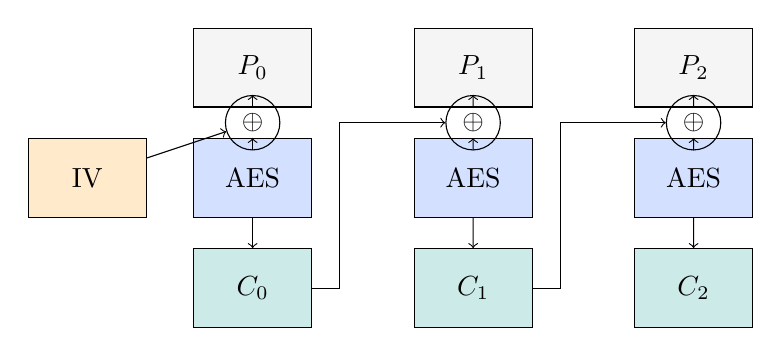
\begin{tikzpicture}[scale=0.7]
    % Blocks
    \foreach \i in {0,1,2} {
        \node[draw, fill=lightgray, minimum width=1.5cm, minimum height=1cm] (p\i) at (\i*4, 2) {$P_\i$};
        \node[draw, fill=primaryblue!20, minimum width=1.5cm, minimum height=1cm] (e\i) at (\i*4, 0) {AES};
        \node[draw, fill=secondarygreen!20, minimum width=1.5cm, minimum height=1cm] (c\i) at (\i*4, -2) {$C_\i$};
        \node[circle, draw, minimum size=0.5cm] (xor\i) at (\i*4, 1) {$\oplus$};
    }
    
    % IV
    \node[draw, fill=accentorange!20, minimum width=1.5cm, minimum height=1cm] (iv) at (-3, 0) {IV};
    
    % Arrows
    \draw[->] (iv) -- (xor0);
    \draw[->] (p0) -- (xor0);
    \draw[->] (xor0) -- (e0);
    \draw[->] (e0) -- (c0);
    
    \foreach \i/\j in {0/1, 1/2} {
        \draw[->] (p\j) -- (xor\j);
        \draw[->] (xor\j) -- (e\j);
        \draw[->] (e\j) -- (c\j);
        \draw[->] (c\i.east) -- ++(0.5,0) |- (xor\j.west);
    }
\end{tikzpicture}
\end{center}

\begin{itemize}
    \item \textbf{IV} (Initialization Vector): Random vector for the first block
    \item Each block depends on the previous block $\Rightarrow$ more security
\end{itemize}

\subsection{Python Code - Symmetric Encryption}

\begin{lstlisting}[language=Python]
from cryptography.hazmat.primitives.ciphers import Cipher, algorithms, modes
import os

# Generate a 256-bit AES key
key = os.urandom(32)

# Generate a random IV
iv = os.urandom(16)

# Create AES-CBC cipher
cipher = Cipher(algorithms.AES(key), modes.CBC(iv))

# Encrypt
encryptor = cipher.encryptor()
ciphertext = encryptor.update(padded_data) + encryptor.finalize()

# Decrypt
decryptor = cipher.decryptor()
plaintext = decryptor.update(ciphertext) + decryptor.finalize()
\end{lstlisting}

% ============================================================
% ASYMMETRIC ENCRYPTION
% ============================================================
\section{Asymmetric Encryption}

\subsection{Principle}

Asymmetric encryption uses \textbf{two different keys}:
\begin{itemize}
    \item \textbf{Public Key}: Shared with everyone, used to \textbf{encrypt}
    \item \textbf{Private Key}: Kept secret, used to \textbf{decrypt}
\end{itemize}

\begin{center}
\begin{tikzpicture}[node distance=2cm, auto]
    % Styles
    \tikzstyle{block} = [rectangle, draw, fill=primaryblue!20, text width=2.5cm, text centered, rounded corners, minimum height=1cm]
    \tikzstyle{pubkey} = [circle, draw, fill=secondarygreen!30, minimum size=1cm]
    \tikzstyle{privkey} = [circle, draw, fill=accentorange!30, minimum size=1cm]
    \tikzstyle{arrow} = [thick,->,>=stealth]
    
    % Nodes
    \node[block] (plain1) {Plaintext};
    \node[pubkey, right=1.5cm of plain1] (enc) {\faUnlock};
    \node[block, right=1.5cm of enc] (cipher) {Ciphertext};
    \node[privkey, right=1.5cm of cipher] (dec) {\faLock};
    \node[block, right=1.5cm of dec] (plain2) {Plaintext};
    
    % Labels
    \node[above=0.3cm of enc] {\small Encryption};
    \node[above=0.3cm of dec] {\small Decryption};
    \node[below=0.3cm of enc] {\textcolor{secondarygreen}{\small Public Key}};
    \node[below=0.3cm of dec] {\textcolor{accentorange}{\small Private Key}};
    
    % Arrows
    \draw[arrow] (plain1) -- (enc);
    \draw[arrow] (enc) -- (cipher);
    \draw[arrow] (cipher) -- (dec);
    \draw[arrow] (dec) -- (plain2);
\end{tikzpicture}
\end{center}

\subsection{RSA Algorithm}

RSA (Rivest-Shamir-Adleman) is based on the difficulty of factoring large prime numbers.

\begin{conceptbox}{RSA Mathematics}
\textbf{Key Generation:}
\begin{enumerate}
    \item Choose two large prime numbers $p$ and $q$
    \item Calculate $n = p \times q$
    \item Calculate $\phi(n) = (p-1)(q-1)$
    \item Choose $e$ such that $\gcd(e, \phi(n)) = 1$ (usually $e = 65537$)
    \item Calculate $d = e^{-1} \mod \phi(n)$
\end{enumerate}

\textbf{Keys:}
\begin{itemize}
    \item Public key: $(n, e)$
    \item Private key: $(n, d)$
\end{itemize}

\textbf{Operations:}
\begin{align*}
    \text{Encryption: } & C = M^e \mod n \\
    \text{Decryption: } & M = C^d \mod n
\end{align*}
\end{conceptbox}

\subsection{OAEP Padding}

For more security, RSA uses \textbf{OAEP} (Optimal Asymmetric Encryption Padding):

\begin{itemize}
    \item Adds randomness to the message
    \item Protects against chosen-ciphertext attacks
    \item Uses hash functions (SHA-256)
\end{itemize}

\subsection{Python Code - Asymmetric Encryption}

\begin{lstlisting}[language=Python]
from cryptography.hazmat.primitives.asymmetric import rsa, padding
from cryptography.hazmat.primitives import hashes

# Generate a 2048-bit RSA key pair
private_key = rsa.generate_private_key(
    public_exponent=65537,
    key_size=2048
)
public_key = private_key.public_key()

# Encrypt with public key
ciphertext = public_key.encrypt(
    message,
    padding.OAEP(
        mgf=padding.MGF1(algorithm=hashes.SHA256()),
        algorithm=hashes.SHA256(),
        label=None
    )
)

# Decrypt with private key
plaintext = private_key.decrypt(ciphertext, padding.OAEP(...))
\end{lstlisting}

% ============================================================
% COMPARISON
% ============================================================
\section{Comparison: Symmetric vs Asymmetric}

\begin{center}
\begin{tabular}{|l|c|c|}
\hline
\rowcolor{primaryblue!30}
\textbf{Criteria} & \textbf{Symmetric} & \textbf{Asymmetric} \\
\hline
\rowcolor{lightgray}
Number of Keys & 1 (same key) & 2 (public/private) \\
\hline
Speed & \textcolor{secondarygreen}{Fast} $\bigstar\bigstar\bigstar$ & \textcolor{red}{Slow} $\bigstar$ \\
\hline
\rowcolor{lightgray}
Key Size & 128-256 bits & 2048-4096 bits \\
\hline
Key Exchange & \textcolor{red}{Difficult} & \textcolor{secondarygreen}{Easy} \\
\hline
\rowcolor{lightgray}
Max Data Size & Unlimited & ~190 bytes (RSA-2048) \\
\hline
Algorithms & AES, DES, 3DES & RSA, ECC, DSA \\
\hline
\rowcolor{lightgray}
Use Cases & Files, Disks & Signatures, HTTPS \\
\hline
\end{tabular}
\end{center}

\subsection{Advantages and Disadvantages}

\begin{minipage}[t]{0.48\textwidth}
\begin{tcolorbox}[colback=secondarygreen!10, colframe=secondarygreen, title=\textbf{Symmetric}]
\textbf{Advantages:}
\begin{itemize}
    \item[$\checkmark$] Very fast
    \item[$\checkmark$] Efficient for large volumes
    \item[$\checkmark$] Short keys
\end{itemize}
\textbf{Disadvantages:}
\begin{itemize}
    \item[$\times$] Key exchange is difficult
    \item[$\times$] Complex key management
\end{itemize}
\end{tcolorbox}
\end{minipage}
\hfill
\begin{minipage}[t]{0.48\textwidth}
\begin{tcolorbox}[colback=primaryblue!10, colframe=primaryblue, title=\textbf{Asymmetric}]
\textbf{Advantages:}
\begin{itemize}
    \item[$\checkmark$] Secure key exchange
    \item[$\checkmark$] Digital signatures
    \item[$\checkmark$] Non-repudiation
\end{itemize}
\textbf{Disadvantages:}
\begin{itemize}
    \item[$\times$] Slow
    \item[$\times$] Long keys
    \item[$\times$] Size limit
\end{itemize}
\end{tcolorbox}
\end{minipage}

% ============================================================
% DEMONSTRATION
% ============================================================
\section{Practical Demonstration}

\subsection{Scenario}

In our demonstration, we:

\begin{enumerate}
    \item \textbf{Created a confidential file}: \texttt{original\_file.txt}
    \item \textbf{Encrypted the file} with AES (symmetric) $\Rightarrow$ \texttt{encrypted\_file.txt}
    \item \textbf{Decrypted the file} $\Rightarrow$ \texttt{decrypted\_file.txt}
\end{enumerate}

\subsection{Results}

\begin{tcolorbox}[colback=lightgray, colframe=darkgray, title=\textbf{Original File}]
\begin{verbatim}
============================================
CONFIDENTIAL FILE
============================================
Name: Ahmed Dinari
Subject: Security Lab Work
Date: November 2025
\end{verbatim}
\end{tcolorbox}

\begin{tcolorbox}[colback=red!5, colframe=red!70, title=\textbf{Encrypted File (Unreadable)}]
\begin{verbatim}
tlJzhikFecZWMIfhqcXY12iKbn/AfPiXSa5dvu
onT2zmEflP0N6/TlZV8SU3+11CrClSc7oZkEZr
55XG8Xkl2wQy...
\end{verbatim}
\end{tcolorbox}

\begin{tcolorbox}[colback=secondarygreen!10, colframe=secondarygreen, title=\textbf{Decrypted File (Same as Original)}]
\begin{verbatim}
============================================
CONFIDENTIAL FILE
============================================
Name: Ahmed Dinari
Subject: Security Lab Work
Date: November 2025
\end{verbatim}
\end{tcolorbox}

% ============================================================
% HYBRID ENCRYPTION
% ============================================================
\section{Hybrid Encryption (Real-World Usage)}

In practice, both methods are combined:

\begin{center}
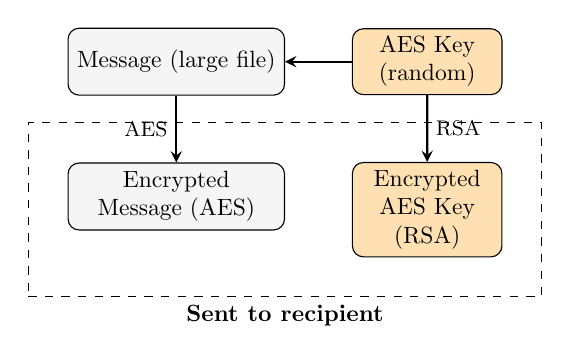
\begin{tikzpicture}[node distance=1.5cm, auto, scale=0.85, transform shape]
    \tikzstyle{block} = [rectangle, draw, fill=lightgray, text width=3cm, text centered, rounded corners, minimum height=1cm]
    \tikzstyle{key} = [rectangle, draw, fill=accentorange!30, text width=2cm, text centered, rounded corners]
    \tikzstyle{arrow} = [thick,->,>=stealth]
    
    % Step 1
    \node[block] (msg) {Message (large file)};
    \node[key, right=1cm of msg] (aeskey) {AES Key (random)};
    
    % Step 2
    \node[block, below=1cm of msg] (encrypted) {Encrypted Message (AES)};
    \node[key, below=1cm of aeskey] (enckey) {Encrypted AES Key (RSA)};
    
    % Arrows
    \draw[arrow] (msg) -- node[left] {\small AES} (encrypted);
    \draw[arrow] (aeskey) -- (msg);
    \draw[arrow] (aeskey) -- node[right] {\small RSA} (enckey);
    
    % Transmission
    \node[draw, dashed, fit=(encrypted)(enckey), inner sep=0.5cm, label=below:{\textbf{Sent to recipient}}] {};
\end{tikzpicture}
\end{center}

\begin{importantbox}
\textbf{Example: HTTPS (TLS/SSL)}
\begin{enumerate}
    \item The server sends its \textbf{RSA public key}
    \item The client generates a \textbf{random AES key}
    \item The client \textbf{encrypts the AES key} with RSA and sends it
    \item All data is \textbf{encrypted with AES}
\end{enumerate}
$\Rightarrow$ Combining the \textbf{speed of AES} with the \textbf{security of RSA}!
\end{importantbox}

% ============================================================
% CONCLUSION
% ============================================================
\section{Conclusion}

\begin{center}
\begin{tikzpicture}
    \node[draw, rounded corners, fill=primaryblue!10, text width=14cm, align=center, inner sep=1cm] {
        \Large\textbf{Key Takeaways}
        
        \vspace{0.5cm}
        
        \begin{tabular}{cl}
            \faKey & \textbf{Symmetric}: 1 key, fast, for files \\[0.3cm]
            \faLock & \textbf{Asymmetric}: 2 keys, secure, for key exchange \\[0.3cm]
            \faShield* & \textbf{Hybrid}: Combines both (HTTPS, Email) \\
        \end{tabular}
    };
\end{tikzpicture}
\end{center}

\vspace{1cm}

\begin{center}
    \Large\textcolor{primaryblue}{\textbf{Thank you for your attention!}}
    
    \vspace{0.5cm}
    
    \normalsize Questions?
\end{center}

\end{document}
